\section{Step 4: Can it perform?}
\begin{frame}{Let's Check: Secure Handwritten Digit Classification as a Service - Demo}
  \begin{columns}[c]
    \begin{column}{0.7\linewidth}
      \begin{figure}[H]
        \centering
        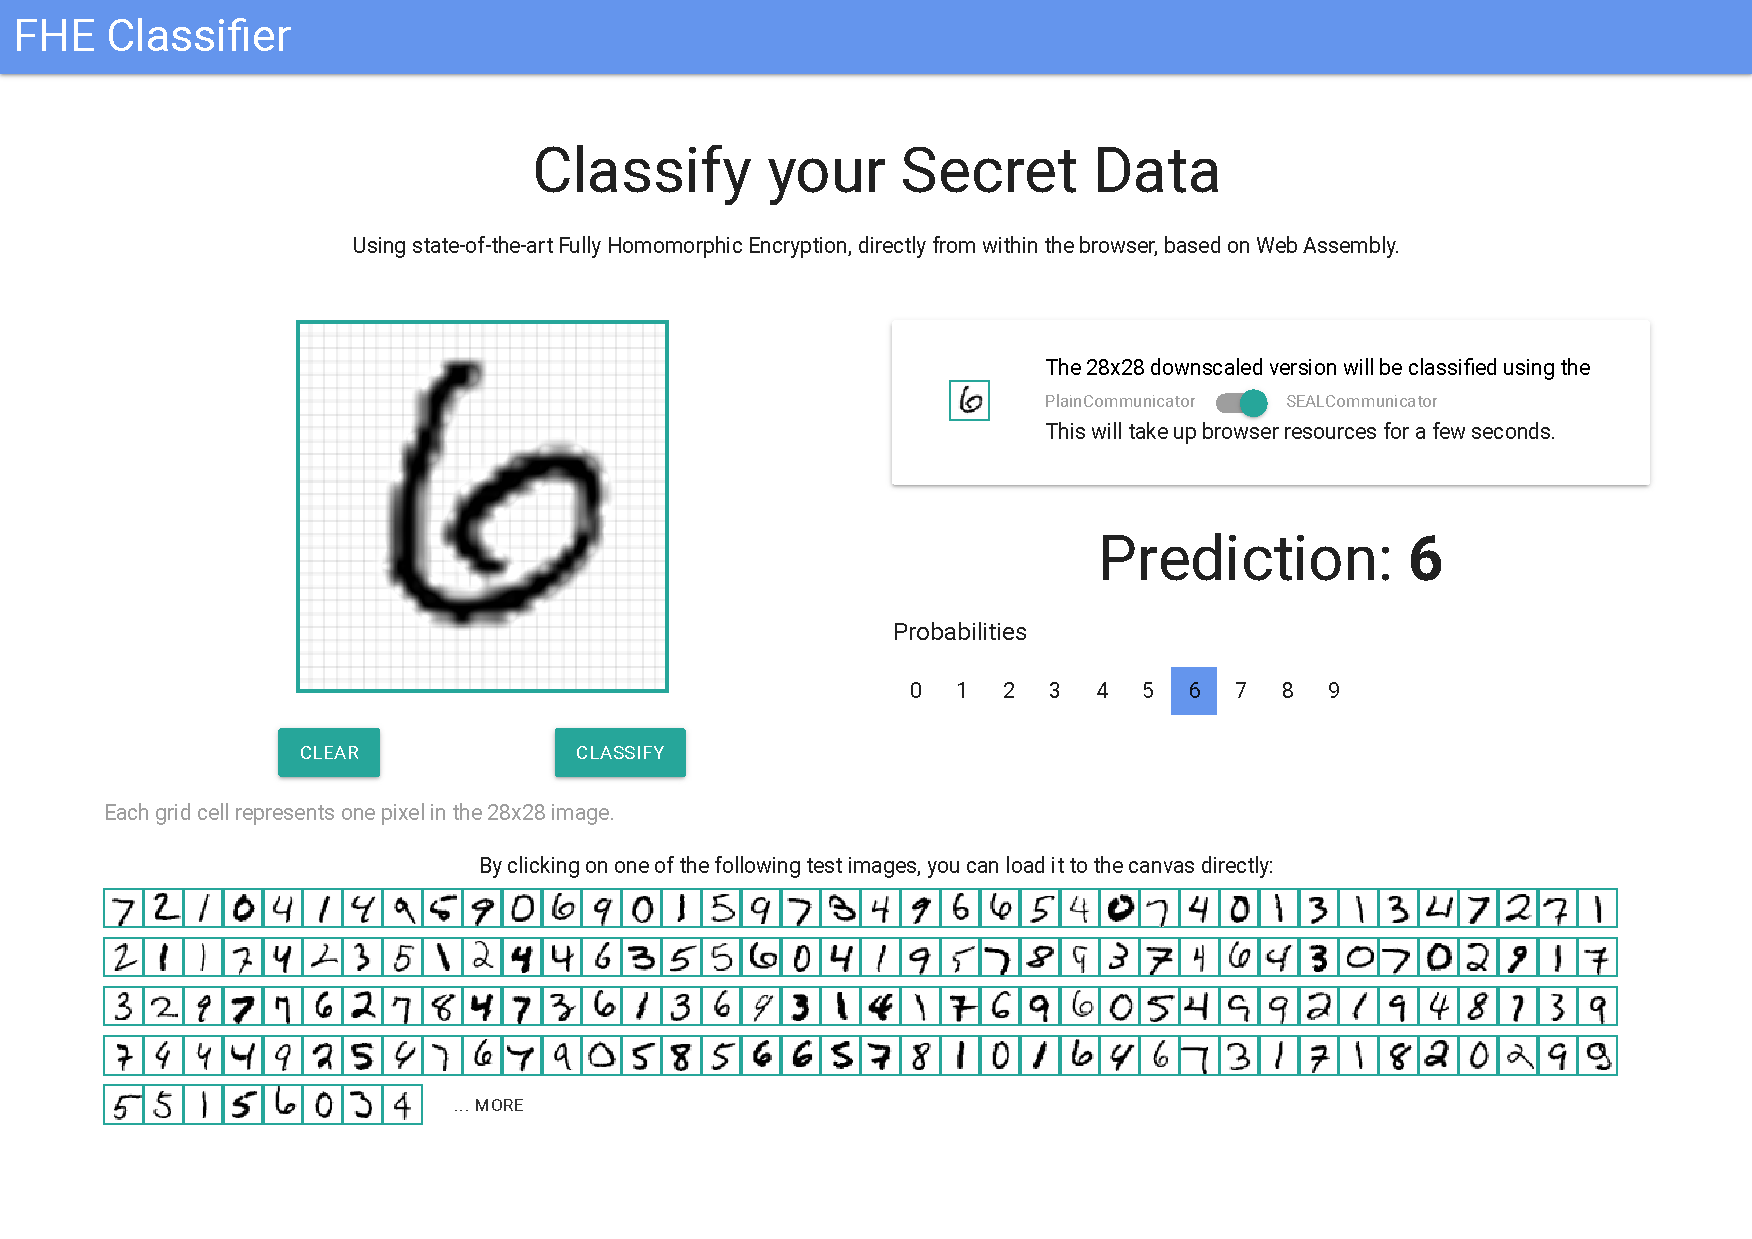
\includegraphics[width=0.75\linewidth]{../thesis/figures/frontend.pdf}
        \vspace{-0.3cm}
        \caption{\url{https://secure-classification.peter.waldert.at/}.}
      \end{figure}
    \end{column}
    \begin{column}{0.24\linewidth}
      Scan the QR-Code:
      \qrcode[nolink,height=3.1cm]{https://secure-classification.peter.waldert.at/}
    \end{column}
  \end{columns}
\end{frame}

\newcommand{\matmulscale}{0.75}
\newcommand{\matmulhoffset}{-3cm}
\begin{frame}{Matrix Multiplication: The Naïve Method}
  \begin{figure}[H]
    \centering
    \hspace{\matmulhoffset}
    \scalebox{\matmulscale}{\inputtikz{figures/generated/matmul-naive}}
    % \caption[Naïve matrix multiplication method]{The naïve method to multiply a matrix $M \in \R^{s \times t}$ with a vector $\vec{x} \in \R^t$ (adapted from \cite{2018-gazelle}).}
    \label{fig:naive-method}
  \end{figure}

  $$\{M \vec{x}\}_i = \sum_{j=1}^{t} M_{ij} x_j \,.$$

  \begin{flushright}\tiny Image adapted from \cite{2020-cryptotree}.\end{flushright}
\end{frame}

\begin{frame}{Matrix Multiplication: The Diagonal Method}
  \begin{figure}[H]
    \centering
    \hspace{\matmulhoffset}
    \scalebox{\matmulscale}{\inputtikz{figures/generated/matmul-diagonal}}
    % \caption[Diagonal matrix multiplication method]{The diagonal method to multiply a square matrix with a vector (adapted from \cite{2018-gazelle}).}
    \label{fig:diagonal-method}
  \end{figure}

  $$M \vec{x} = \sum_{j=0}^{t-1} \diag_j(M) \cdot \rot_j(\vec{x}) \,.$$

  \begin{flushright}\tiny Image adapted from \cite{2020-cryptotree}.\end{flushright}
\end{frame}

\begin{frame}{Matrix Multiplication: The Hybrid Method}
  \begin{figure}[H]
    \centering
    \hspace{\matmulhoffset}
    \scalebox{\matmulscale}{\inputtikz{figures/generated/matmul-hybrid}}
    % \caption[Hybrid matrix multiplication method]{The hybrid method to multiply an arbitrarily sized matrix with a vector (adapted from \cite{2018-gazelle}).}
    \label{fig:hybrid-method}
  \end{figure}

  $$M \vec{x} = (y_i)_{i \in \Z/s\Z} \;\text{with}\; \vec{y} = \sum_{k=1}^{t / s} \rot_{ks}\bigg(\sum_{j=1}^s \diag_j(M) \cdot \rot_j(\vec{x})\bigg) \,.$$

  \begin{flushright}\tiny Image adapted from \cite{2020-cryptotree}.\end{flushright}
\end{frame}

\begin{frame}{Polynomial Evaluation}
  \begin{itemize}
    \item In between the dense layers, we need to evaluate the $\cryptop{relu}(x) := \max(x, 0)$ function. \\
          $\Rightarrow$ Approximate it by a series expansion...
          $$\cryptop{relu\_taylor}(x) = -0.006137 x^3 + 0.090189 x^2 + 0.59579 x + 0.54738 \,.$$
    \item The \cryptop{softmax} activation at the end can be done by the client.
  \end{itemize}

  \begin{figure}[H]
    \centering
    \scalebox{0.56}{\inputtikz{figures/generated/taylor-relu}}
    \label{fig:taylor-relu}
  \end{figure}
\end{frame}

\begin{frame}{Runtime Benchmarks \& Communication Overhead}
  \begin{table}[H]
    \centering
    \setlength{\belowcaptionskip}{0pt}
    \caption[Performance Benchmarks / Communication Overhead]{
      Performance benchmarks and communication overhead of the classification procedure on an Intel\textregistered \, i7-5600U CPU, including the encoding and decoding steps.
      \vspace{-0.2cm}
    }
    % \captionsetup{margin=10pt}
    % \caption*{
    %   $\bm{B_1}$ ... Coefficient Moduli start bits (also equal to the last) \\
    %   $\bm{B_2}$ ... Coefficient Moduli middle bits, also defines the scale as $2^{B_2}$ \\
    %   $\bm{N}$ ... Polynomial Modulus Degree, found in the exponent of $p(X) = X^N + 1$ \\
    %   $\bm{T}$ ... Runtime of encryption + classification + decryption \\
    %   $\bm{M}$ ... Message Size (Relin Keys + Galois Keys + Request Ciphertext + Response Ciphertext) \\
    %   $\bm{\Delta}$ ... Mean Max-Relative Error compared to the exact result, i.e. $\bm{\Delta} := \frac{\langle |\bm{y}_{prediction} - \bm{y}_{exact}| \rangle}{\max |\bm{y}_{exact}|}$
    % }
    \SetTblrInner{rowsep=1pt}
    \scalebox{0.8}{
      \begin{tblr}{
        colspec={ccrrrr|rrr},
        row{2,3,4} = {bg=azure9},
        row{5,6,7} = {bg=violet9},
        row{8,9,10} = {bg=blue9},
        row{11,12,13} = {bg=azure9},
          }
        \hline
        \bf Mode & \bf SecLevel & $\bm{B_1}$ & $\bm{B_2}$ & $\bm{N}$ & \bf MatMul & $\bm{T}$ / \si{\second} & $\bm{M}$ / \si{\mebi\byte} & $\bm{\Delta}$ / 1 \\
        \hline
        & & & & & Diagonal & 8.39 & 132.72 & 0.0364 \\
        Release & tc128 & 34 & 25 & 8192 & Hybrid & 1.35 & 132.72 & 0.0362 \\
        & & & & & BSGS & 1.66 & 132.72 & 0.1433 \\
        \hline
        & & & & & Diagonal & 17.24 & 286.51 & 0.0363 \\
        & tc128 & 60 & 40 & 16384 & Hybrid & 3.05 & 286.51 & 0.0364 \\
        & & & & & BSGS & 3.66 & 286.51 & 0.1399 \\
        \hline
        & & & & & Diagonal & 35.24 & 615.16 & 0.0363 \\
        & tc256 & 60 & 40 & 32768& Hybrid & 5.99 & 615.16 & 0.0364 \\
        & & & & & BSGS & 7.34 & 615.16 & 0.1399 \\
      \end{tblr}
    }
    \label{tab:performance-benchmarks}
  \end{table}
  In Plain: 784 byte requests, taking \SI{50}{\micro\second}; Encrypted: \SI{132}{\mebi\byte} requests, taking \SI{1.4}{\second}.
\end{frame}
